\documentclass[1p]{elsarticle_modified}
%\bibliographystyle{elsarticle-num}

%\usepackage[colorlinks]{hyperref}
%\usepackage{abbrmath_seonhwa} %\Abb, \Ascr, \Acal ,\Abf, \Afrak
\usepackage{amsfonts}
\usepackage{amssymb}
\usepackage{amsmath}
\usepackage{amsthm}
\usepackage{scalefnt}
\usepackage{amsbsy}
\usepackage{kotex}
\usepackage{caption}
\usepackage{subfig}
\usepackage{color}
\usepackage{graphicx}
\usepackage{xcolor} %% white, black, red, green, blue, cyan, magenta, yellow
\usepackage{float}
\usepackage{setspace}
\usepackage{hyperref}

\usepackage{tikz}
\usetikzlibrary{arrows}

\usepackage{multirow}
\usepackage{array} % fixed length table
\usepackage{hhline}

%%%%%%%%%%%%%%%%%%%%%
\makeatletter
\renewcommand*\env@matrix[1][\arraystretch]{%
	\edef\arraystretch{#1}%
	\hskip -\arraycolsep
	\let\@ifnextchar\new@ifnextchar
	\array{*\c@MaxMatrixCols c}}
\makeatother %https://tex.stackexchange.com/questions/14071/how-can-i-increase-the-line-spacing-in-a-matrix
%%%%%%%%%%%%%%%

\usepackage[normalem]{ulem}

\newcommand{\msout}[1]{\ifmmode\text{\sout{\ensuremath{#1}}}\else\sout{#1}\fi}
%SOURCE: \msout is \stkout macro in https://tex.stackexchange.com/questions/20609/strikeout-in-math-mode

\newcommand{\cancel}[1]{
	\ifmmode
	{\color{red}\msout{#1}}
	\else
	{\color{red}\sout{#1}}
	\fi
}

\newcommand{\add}[1]{
	{\color{blue}\uwave{#1}}
}

\newcommand{\replace}[2]{
	\ifmmode
	{\color{red}\msout{#1}}{\color{blue}\uwave{#2}}
	\else
	{\color{red}\sout{#1}}{\color{blue}\uwave{#2}}
	\fi
}

\newcommand{\Sol}{\mathcal{S}} %segment
\newcommand{\D}{D} %diagram
\newcommand{\A}{\mathcal{A}} %arc


%%%%%%%%%%%%%%%%%%%%%%%%%%%%%5 test

\def\sl{\operatorname{\textup{SL}}(2,\Cbb)}
\def\psl{\operatorname{\textup{PSL}}(2,\Cbb)}
\def\quan{\mkern 1mu \triangleright \mkern 1mu}

\theoremstyle{definition}
\newtheorem{thm}{Theorem}[section]
\newtheorem{prop}[thm]{Proposition}
\newtheorem{lem}[thm]{Lemma}
\newtheorem{ques}[thm]{Question}
\newtheorem{cor}[thm]{Corollary}
\newtheorem{defn}[thm]{Definition}
\newtheorem{exam}[thm]{Example}
\newtheorem{rmk}[thm]{Remark}
\newtheorem{alg}[thm]{Algorithm}

\newcommand{\I}{\sqrt{-1}}
\begin{document}

%\begin{frontmatter}
%
%\title{Boundary parabolic representations of knots up to 8 crossings}
%
%%% Group authors per affiliation:
%\author{Yunhi Cho} 
%\address{Department of Mathematics, University of Seoul, Seoul, Korea}
%\ead{yhcho@uos.ac.kr}
%
%
%\author{Seonhwa Kim} %\fnref{s_kim}}
%\address{Center for Geometry and Physics, Institute for Basic Science, Pohang, 37673, Korea}
%\ead{ryeona17@ibs.re.kr}
%
%\author{Hyuk Kim}
%\address{Department of Mathematical Sciences, Seoul National University, Seoul 08826, Korea}
%\ead{hyukkim@snu.ac.kr}
%
%\author{Seokbeom Yoon}
%\address{Department of Mathematical Sciences, Seoul National University, Seoul, 08826,  Korea}
%\ead{sbyoon15@snu.ac.kr}
%
%\begin{abstract}
%We find all boundary parabolic representation of knots up to 8 crossings.
%
%\end{abstract}
%\begin{keyword}
%    \MSC[2010] 57M25 
%\end{keyword}
%
%\end{frontmatter}

%\linenumbers
%\tableofcontents
%
\newcommand\colored[1]{\textcolor{white}{\rule[-0.35ex]{0.8em}{1.4ex}}\kern-0.8em\color{red} #1}%
%\newcommand\colored[1]{\textcolor{white}{ #1}\kern-2.17ex	\textcolor{white}{ #1}\kern-1.81ex	\textcolor{white}{ #1}\kern-2.15ex\color{red}#1	}

{\Large $\underline{12a_{1262}~(K12a_{1262})}$}

\setlength{\tabcolsep}{10pt}
\renewcommand{\arraystretch}{1.6}
\vspace{1cm}\begin{tabular}{m{100pt}>{\centering\arraybackslash}m{274pt}}
\multirow{5}{120pt}{
	\centering
	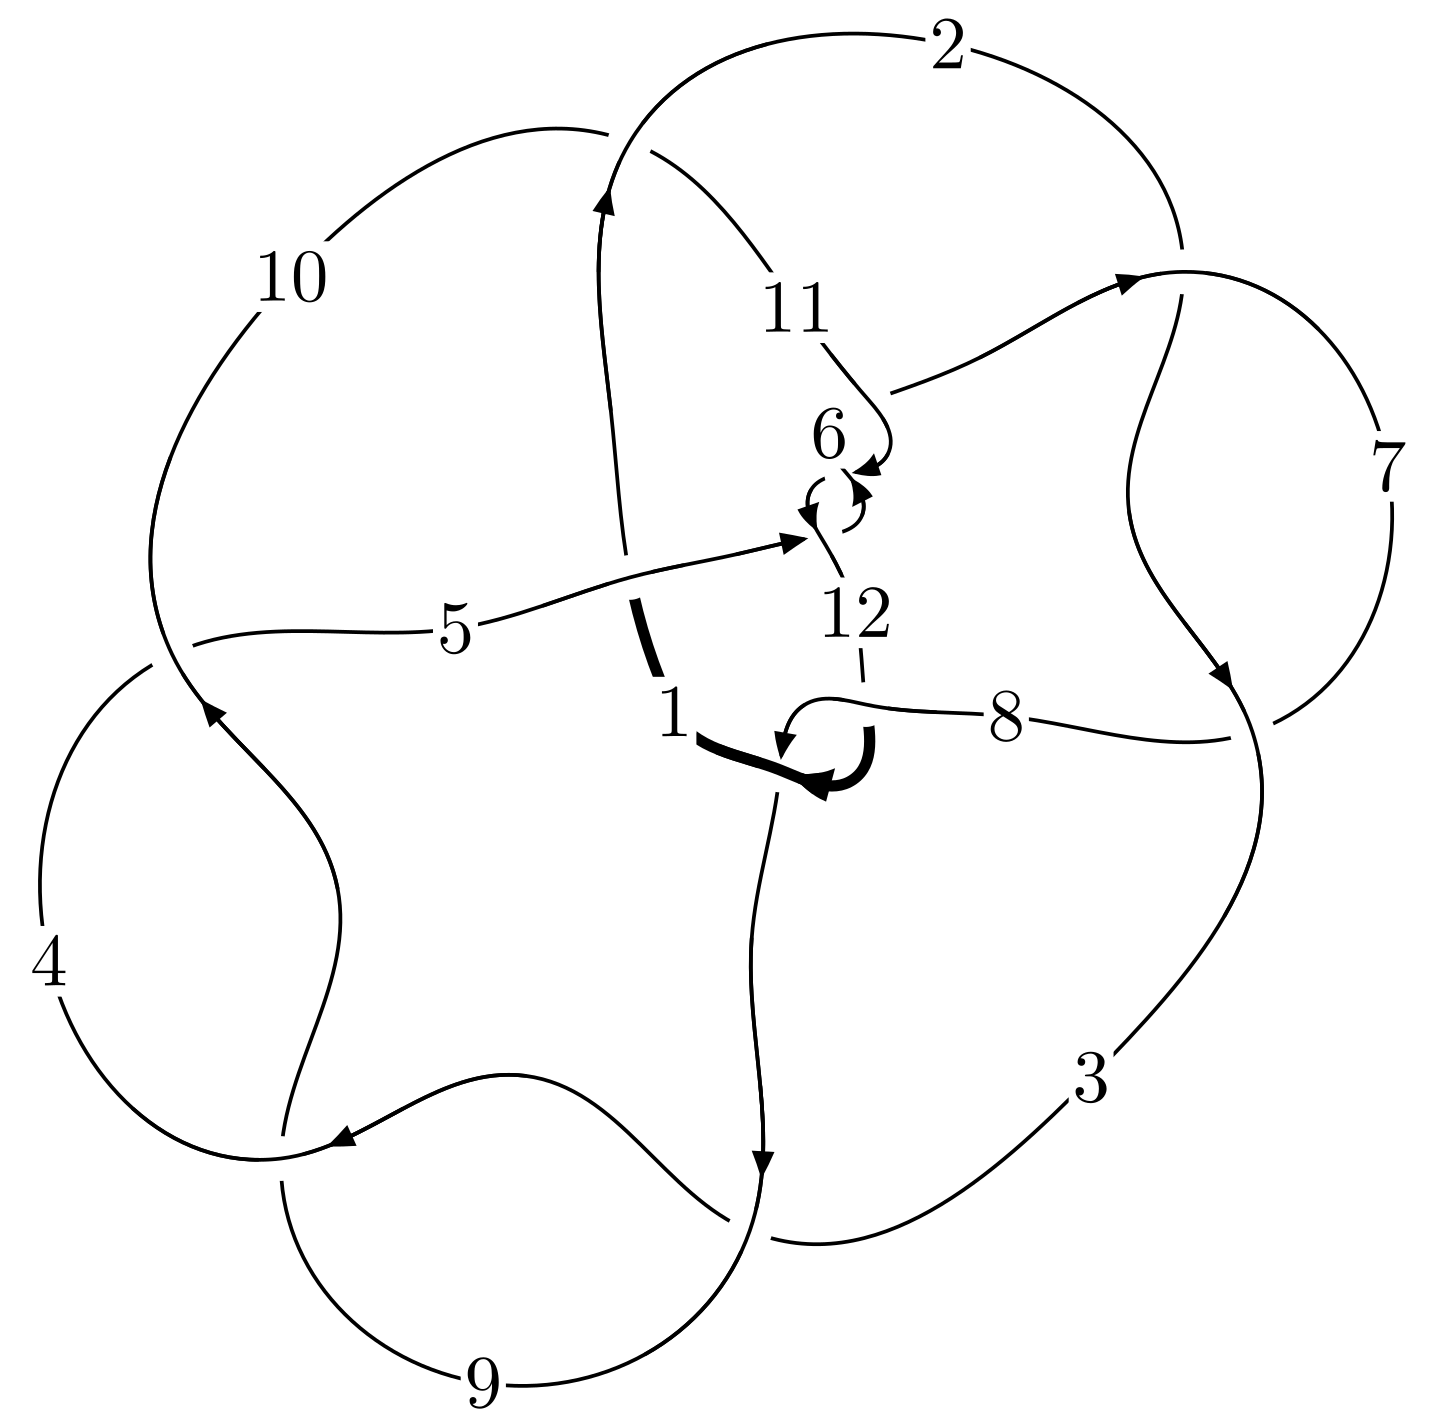
\includegraphics[width=112pt]{../../../GIT/diagram.site/Diagrams/png/2063_12a_1262.png}\\
\ \ \ A knot diagram\footnotemark}&
\allowdisplaybreaks
\textbf{Linearized knot diagam} \\
\cline{2-2}
 &
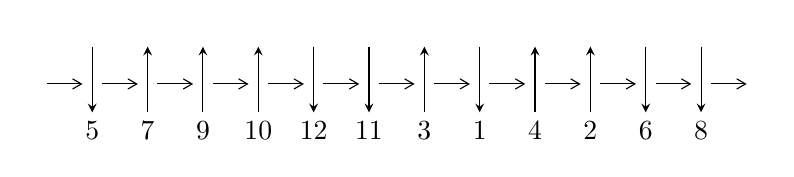
\begin{tikzpicture}[x=20pt, y=17pt]
	% nodes
	\node (C0) at (0, 0) {};
	\node (C1) at (1, 0) {};
	\node (C1U) at (1, +1) {};
	\node (C1D) at (1, -1) {5};

	\node (C2) at (2, 0) {};
	\node (C2U) at (2, +1) {};
	\node (C2D) at (2, -1) {7};

	\node (C3) at (3, 0) {};
	\node (C3U) at (3, +1) {};
	\node (C3D) at (3, -1) {9};

	\node (C4) at (4, 0) {};
	\node (C4U) at (4, +1) {};
	\node (C4D) at (4, -1) {10};

	\node (C5) at (5, 0) {};
	\node (C5U) at (5, +1) {};
	\node (C5D) at (5, -1) {12};

	\node (C6) at (6, 0) {};
	\node (C6U) at (6, +1) {};
	\node (C6D) at (6, -1) {11};

	\node (C7) at (7, 0) {};
	\node (C7U) at (7, +1) {};
	\node (C7D) at (7, -1) {3};

	\node (C8) at (8, 0) {};
	\node (C8U) at (8, +1) {};
	\node (C8D) at (8, -1) {1};

	\node (C9) at (9, 0) {};
	\node (C9U) at (9, +1) {};
	\node (C9D) at (9, -1) {4};

	\node (C10) at (10, 0) {};
	\node (C10U) at (10, +1) {};
	\node (C10D) at (10, -1) {2};

	\node (C11) at (11, 0) {};
	\node (C11U) at (11, +1) {};
	\node (C11D) at (11, -1) {6};

	\node (C12) at (12, 0) {};
	\node (C12U) at (12, +1) {};
	\node (C12D) at (12, -1) {8};
	\node (C13) at (13, 0) {};

	% arrows
	\draw[->,>={angle 60}]
	(C0) edge (C1) (C1) edge (C2) (C2) edge (C3) (C3) edge (C4) (C4) edge (C5) (C5) edge (C6) (C6) edge (C7) (C7) edge (C8) (C8) edge (C9) (C9) edge (C10) (C10) edge (C11) (C11) edge (C12) (C12) edge (C13) ;	\draw[->,>=stealth]
	(C1U) edge (C1D) (C2D) edge (C2U) (C3D) edge (C3U) (C4D) edge (C4U) (C5U) edge (C5D) (C6U) edge (C6D) (C7D) edge (C7U) (C8U) edge (C8D) (C9D) edge (C9U) (C10D) edge (C10U) (C11U) edge (C11D) (C12U) edge (C12D) ;
	\end{tikzpicture} \\
\hhline{~~} \\& 
\textbf{Solving Sequence} \\ \cline{2-2} 
 &
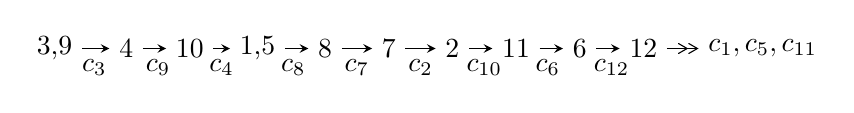
\begin{tikzpicture}[x=23pt, y=7pt]
	% node
	\node (A0) at (-1/8, 0) {3,9};
	\node (A1) at (1, 0) {4};
	\node (A2) at (2, 0) {10};
	\node (A3) at (49/16, 0) {1,5};
	\node (A4) at (33/8, 0) {8};
	\node (A5) at (41/8, 0) {7};
	\node (A6) at (49/8, 0) {2};
	\node (A7) at (57/8, 0) {11};
	\node (A8) at (65/8, 0) {6};
	\node (A9) at (73/8, 0) {12};
	\node (C1) at (1/2, -1) {$c_{3}$};
	\node (C2) at (3/2, -1) {$c_{9}$};
	\node (C3) at (5/2, -1) {$c_{4}$};
	\node (C4) at (29/8, -1) {$c_{8}$};
	\node (C5) at (37/8, -1) {$c_{7}$};
	\node (C6) at (45/8, -1) {$c_{2}$};
	\node (C7) at (53/8, -1) {$c_{10}$};
	\node (C8) at (61/8, -1) {$c_{6}$};
	\node (C9) at (69/8, -1) {$c_{12}$};
	\node (A10) at (11, 0) {$c_{1},c_{5},c_{11}$};

	% edge
	\draw[->,>=stealth]	
	(A0) edge (A1) (A1) edge (A2) (A2) edge (A3) (A3) edge (A4) (A4) edge (A5) (A5) edge (A6) (A6) edge (A7) (A7) edge (A8) (A8) edge (A9) ;
	\draw[->>,>={angle 60}]	
	(A9) edge (A10);
\end{tikzpicture} \\ 

\end{tabular} \\

\footnotetext{
The image of knot diagram is generated by the software ``\textbf{Draw programme}" developed by Andrew Bartholomew(\url{http://www.layer8.co.uk/maths/draw/index.htm\#Running-draw}), where we modified some parts for our purpose(\url{https://github.com/CATsTAILs/LinksPainter}).
}\phantom \\ \newline 
\centering \textbf{Ideals for irreducible components\footnotemark of $X_{\text{par}}$} 
 
\begin{align*}
I^u_{1}&=\langle 
-2.70194\times10^{188} u^{96}+3.19613\times10^{188} u^{95}+\cdots+2.54218\times10^{187} b+3.85233\times10^{188},\\
\phantom{I^u_{1}}&\phantom{= \langle  }2.54426\times10^{188} u^{96}-1.10013\times10^{188} u^{95}+\cdots+2.54218\times10^{187} a-8.55554\times10^{188},\;u^{97}-50 u^{95}+\cdots-4 u-1\rangle \\
I^u_{2}&=\langle 
-592 u^{24}-394 u^{23}+\cdots+559 b-776,\;-25 u^{24}+684 u^{23}+\cdots+559 a+564,\\
\phantom{I^u_{2}}&\phantom{= \langle  }u^{25}-14 u^{23}+\cdots+2 u^2-1\rangle \\
I^u_{3}&=\langle 
b,\;a-1,\;u+1\rangle \\
\\
\end{align*}
\raggedright * 3 irreducible components of $\dim_{\mathbb{C}}=0$, with total 123 representations.\\
\footnotetext{All coefficients of polynomials are rational numbers. But the coefficients are sometimes approximated in decimal forms when there is not enough margin.}
\newpage
\renewcommand{\arraystretch}{1}
\centering \section*{I. $I^u_{1}= \langle -2.70\times10^{188} u^{96}+3.20\times10^{188} u^{95}+\cdots+2.54\times10^{187} b+3.85\times10^{188},\;2.54\times10^{188} u^{96}-1.10\times10^{188} u^{95}+\cdots+2.54\times10^{187} a-8.56\times10^{188},\;u^{97}-50 u^{95}+\cdots-4 u-1 \rangle$}
\flushleft \textbf{(i) Arc colorings}\\
\begin{tabular}{m{7pt} m{180pt} m{7pt} m{180pt} }
\flushright $a_{3}=$&$\begin{pmatrix}1\\0\end{pmatrix}$ \\
\flushright $a_{9}=$&$\begin{pmatrix}0\\u\end{pmatrix}$ \\
\flushright $a_{4}=$&$\begin{pmatrix}1\\- u^2\end{pmatrix}$ \\
\flushright $a_{10}=$&$\begin{pmatrix}u\\- u^3+u\end{pmatrix}$ \\
\flushright $a_{1}=$&$\begin{pmatrix}-10.0082 u^{96}+4.32750 u^{95}+\cdots+48.6803 u+33.6544\\10.6285 u^{96}-12.5724 u^{95}+\cdots-17.7846 u-15.1536\end{pmatrix}$ \\
\flushright $a_{5}=$&$\begin{pmatrix}- u^2+1\\u^4-2 u^2\end{pmatrix}$ \\
\flushright $a_{8}=$&$\begin{pmatrix}12.5922 u^{96}-1.77202 u^{95}+\cdots+14.2481 u-46.7205\\4.63659 u^{96}-4.60135 u^{95}+\cdots-6.79228 u-8.49313\end{pmatrix}$ \\
\flushright $a_{7}=$&$\begin{pmatrix}7.95562 u^{96}+2.82932 u^{95}+\cdots+21.0403 u-38.2274\\4.63659 u^{96}-4.60135 u^{95}+\cdots-6.79228 u-8.49313\end{pmatrix}$ \\
\flushright $a_{2}=$&$\begin{pmatrix}-16.6625 u^{96}+13.0338 u^{95}+\cdots+57.8871 u+41.2971\\9.78142 u^{96}-11.3527 u^{95}+\cdots-14.9995 u-14.6073\end{pmatrix}$ \\
\flushright $a_{11}=$&$\begin{pmatrix}9.03230 u^{96}-6.50457 u^{95}+\cdots+2.34776 u-16.4773\\-1.79403 u^{96}+3.98873 u^{95}+\cdots+18.6428 u-5.18379\end{pmatrix}$ \\
\flushright $a_{6}=$&$\begin{pmatrix}-1.45738 u^{96}+13.6162 u^{95}+\cdots+10.2044 u-23.8542\\0.372455 u^{96}-4.69082 u^{95}+\cdots+3.81710 u+9.83895\end{pmatrix}$ \\
\flushright $a_{12}=$&$\begin{pmatrix}-3.88855 u^{96}+12.2474 u^{95}+\cdots-4.60422 u-15.8760\\2.97130 u^{96}-1.96134 u^{95}+\cdots+0.369519 u-9.54574\end{pmatrix}$\\&\end{tabular}
\flushleft \textbf{(ii) Obstruction class $= -1$}\\~\\
\flushleft \textbf{(iii) Cusp Shapes $= 6.91455 u^{96}-6.40239 u^{95}+\cdots-108.420 u+0.833440$}\\~\\
\newpage\renewcommand{\arraystretch}{1}
\flushleft \textbf{(iv) u-Polynomials at the component}\newline \\
\begin{tabular}{m{50pt}|m{274pt}}
Crossings & \hspace{64pt}u-Polynomials at each crossing \\
\hline $$\begin{aligned}c_{1}\end{aligned}$$&$\begin{aligned}
&u^{97}+8 u^{96}+\cdots+12842088 u-1859089
\end{aligned}$\\
\hline $$\begin{aligned}c_{2},c_{7}\end{aligned}$$&$\begin{aligned}
&u^{97}+u^{96}+\cdots-10909 u-1781
\end{aligned}$\\
\hline $$\begin{aligned}c_{3},c_{4},c_{9}\end{aligned}$$&$\begin{aligned}
&u^{97}-50 u^{95}+\cdots-4 u+1
\end{aligned}$\\
\hline $$\begin{aligned}c_{5},c_{6},c_{11}\end{aligned}$$&$\begin{aligned}
&u^{97}- u^{96}+\cdots+44 u-1
\end{aligned}$\\
\hline $$\begin{aligned}c_{8},c_{12}\end{aligned}$$&$\begin{aligned}
&u^{97}+u^{96}+\cdots+231 u-43
\end{aligned}$\\
\hline $$\begin{aligned}c_{10}\end{aligned}$$&$\begin{aligned}
&u^{97}-6 u^{96}+\cdots-51370688 u+9617432
\end{aligned}$\\
\hline
\end{tabular}\\~\\
\newpage\renewcommand{\arraystretch}{1}
\flushleft \textbf{(v) Riley Polynomials at the component}\newline \\
\begin{tabular}{m{50pt}|m{274pt}}
Crossings & \hspace{64pt}Riley Polynomials at each crossing \\
\hline $$\begin{aligned}c_{1}\end{aligned}$$&$\begin{aligned}
&y^{97}+32 y^{96}+\cdots-39674367994840 y-3456211909921
\end{aligned}$\\
\hline $$\begin{aligned}c_{2},c_{7}\end{aligned}$$&$\begin{aligned}
&y^{97}-85 y^{96}+\cdots+551971 y-3171961
\end{aligned}$\\
\hline $$\begin{aligned}c_{3},c_{4},c_{9}\end{aligned}$$&$\begin{aligned}
&y^{97}-100 y^{96}+\cdots+80 y-1
\end{aligned}$\\
\hline $$\begin{aligned}c_{5},c_{6},c_{11}\end{aligned}$$&$\begin{aligned}
&y^{97}+103 y^{96}+\cdots+2246 y-1
\end{aligned}$\\
\hline $$\begin{aligned}c_{8},c_{12}\end{aligned}$$&$\begin{aligned}
&y^{97}-47 y^{96}+\cdots+27905 y-1849
\end{aligned}$\\
\hline $$\begin{aligned}c_{10}\end{aligned}$$&$\begin{aligned}
&y^{97}-54 y^{96}+\cdots+2993028924913184 y-92494998274624
\end{aligned}$\\
\hline
\end{tabular}\\~\\
\newpage\flushleft \textbf{(vi) Complex Volumes and Cusp Shapes}
$$\begin{array}{c|c|c}  
\text{Solutions to }I^u_{1}& \I (\text{vol} + \sqrt{-1}CS) & \text{Cusp shape}\\
 \hline 
\begin{aligned}
u &= \phantom{-}0.392511 + 0.929569 I \\
a &= -0.119570 - 1.045380 I \\
b &= -0.80861 - 1.61190 I\end{aligned}
 & \phantom{-}1.66027 + 2.03268 I & \phantom{-0.000000 } 0 \\ \hline\begin{aligned}
u &= \phantom{-}0.392511 - 0.929569 I \\
a &= -0.119570 + 1.045380 I \\
b &= -0.80861 + 1.61190 I\end{aligned}
 & \phantom{-}1.66027 - 2.03268 I & \phantom{-0.000000 } 0 \\ \hline\begin{aligned}
u &= \phantom{-}0.517075 + 0.869044 I \\
a &= -0.003713 - 1.342650 I \\
b &= -0.76665 - 1.62978 I\end{aligned}
 & \phantom{-}8.2073 + 12.3283 I & \phantom{-0.000000 } 0 \\ \hline\begin{aligned}
u &= \phantom{-}0.517075 - 0.869044 I \\
a &= -0.003713 + 1.342650 I \\
b &= -0.76665 + 1.62978 I\end{aligned}
 & \phantom{-}8.2073 - 12.3283 I & \phantom{-0.000000 } 0 \\ \hline\begin{aligned}
u &= -0.495647 + 0.905002 I \\
a &= \phantom{-}0.002226 + 1.194820 I \\
b &= -0.79748 + 1.60970 I\end{aligned}
 & \phantom{-}1.27001 - 7.95601 I & \phantom{-0.000000 } 0 \\ \hline\begin{aligned}
u &= -0.495647 - 0.905002 I \\
a &= \phantom{-}0.002226 - 1.194820 I \\
b &= -0.79748 - 1.60970 I\end{aligned}
 & \phantom{-}1.27001 + 7.95601 I & \phantom{-0.000000 } 0 \\ \hline\begin{aligned}
u &= -0.956296\phantom{ +0.000000I} \\
a &= \phantom{-}0.992260\phantom{ +0.000000I} \\
b &= \phantom{-}0.0790206\phantom{ +0.000000I}\end{aligned}
 & \phantom{-}1.64464\phantom{ +0.000000I} & \phantom{-0.000000 } 0 \\ \hline\begin{aligned}
u &= \phantom{-}0.877270 + 0.316407 I \\
a &= \phantom{-}1.263720 + 0.169632 I \\
b &= \phantom{-}0.380432 - 0.262755 I\end{aligned}
 & \phantom{-}6.91275 + 0.04134 I & \phantom{-0.000000 } 0 \\ \hline\begin{aligned}
u &= \phantom{-}0.877270 - 0.316407 I \\
a &= \phantom{-}1.263720 - 0.169632 I \\
b &= \phantom{-}0.380432 + 0.262755 I\end{aligned}
 & \phantom{-}6.91275 - 0.04134 I & \phantom{-0.000000 } 0 \\ \hline\begin{aligned}
u &= \phantom{-}0.683668 + 0.839515 I \\
a &= -1.001000 + 0.353649 I \\
b &= -0.093482 + 1.226850 I\end{aligned}
 & \phantom{-}8.65876 - 6.63877 I & \phantom{-0.000000 } 0\\
 \hline 
 \end{array}$$\newpage$$\begin{array}{c|c|c}  
\text{Solutions to }I^u_{1}& \I (\text{vol} + \sqrt{-1}CS) & \text{Cusp shape}\\
 \hline 
\begin{aligned}
u &= \phantom{-}0.683668 - 0.839515 I \\
a &= -1.001000 - 0.353649 I \\
b &= -0.093482 - 1.226850 I\end{aligned}
 & \phantom{-}8.65876 + 6.63877 I & \phantom{-0.000000 } 0 \\ \hline\begin{aligned}
u &= -1.046750 + 0.387787 I \\
a &= \phantom{-}0.830817 + 0.465873 I \\
b &= -1.275660 + 0.578401 I\end{aligned}
 & \phantom{-}1.30768 - 4.06870 I & \phantom{-0.000000 } 0 \\ \hline\begin{aligned}
u &= -1.046750 - 0.387787 I \\
a &= \phantom{-}0.830817 - 0.465873 I \\
b &= -1.275660 - 0.578401 I\end{aligned}
 & \phantom{-}1.30768 + 4.06870 I & \phantom{-0.000000 } 0 \\ \hline\begin{aligned}
u &= -0.803486 + 0.809664 I \\
a &= -0.799371 - 0.188894 I \\
b &= \phantom{-}0.102850 - 1.189290 I\end{aligned}
 & \phantom{-}2.11438 + 2.11101 I & \phantom{-0.000000 } 0 \\ \hline\begin{aligned}
u &= -0.803486 - 0.809664 I \\
a &= -0.799371 + 0.188894 I \\
b &= \phantom{-}0.102850 + 1.189290 I\end{aligned}
 & \phantom{-}2.11438 - 2.11101 I & \phantom{-0.000000 } 0 \\ \hline\begin{aligned}
u &= \phantom{-}0.716315 + 0.458579 I \\
a &= -0.678169 - 0.485281 I \\
b &= \phantom{-}0.189753 + 0.681947 I\end{aligned}
 & \phantom{-}3.34504 + 3.10873 I & \phantom{-0.000000 } 0 \\ \hline\begin{aligned}
u &= \phantom{-}0.716315 - 0.458579 I \\
a &= -0.678169 + 0.485281 I \\
b &= \phantom{-}0.189753 - 0.681947 I\end{aligned}
 & \phantom{-}3.34504 - 3.10873 I & \phantom{-0.000000 } 0 \\ \hline\begin{aligned}
u &= -0.325366 + 0.768932 I \\
a &= -0.347414 + 1.034470 I \\
b &= -0.88331 + 1.57712 I\end{aligned}
 & \phantom{-}9.59958 + 1.86764 I & \phantom{-0.000000 } 0 \\ \hline\begin{aligned}
u &= -0.325366 - 0.768932 I \\
a &= -0.347414 - 1.034470 I \\
b &= -0.88331 - 1.57712 I\end{aligned}
 & \phantom{-}9.59958 - 1.86764 I & \phantom{-0.000000 } 0 \\ \hline\begin{aligned}
u &= -0.550305 + 0.584327 I \\
a &= -1.308720 + 0.502260 I \\
b &= -0.111757 - 0.693519 I\end{aligned}
 & \phantom{-}10.46470 - 6.14501 I & \phantom{-0.000000 } 0\\
 \hline 
 \end{array}$$\newpage$$\begin{array}{c|c|c}  
\text{Solutions to }I^u_{1}& \I (\text{vol} + \sqrt{-1}CS) & \text{Cusp shape}\\
 \hline 
\begin{aligned}
u &= -0.550305 - 0.584327 I \\
a &= -1.308720 - 0.502260 I \\
b &= -0.111757 + 0.693519 I\end{aligned}
 & \phantom{-}10.46470 + 6.14501 I & \phantom{-0.000000 } 0 \\ \hline\begin{aligned}
u &= \phantom{-}1.100200 + 0.482089 I \\
a &= -0.416480 + 0.017263 I \\
b &= \phantom{-}0.574249 + 1.010610 I\end{aligned}
 & \phantom{-}3.52627 + 3.19540 I & \phantom{-0.000000 } 0 \\ \hline\begin{aligned}
u &= \phantom{-}1.100200 - 0.482089 I \\
a &= -0.416480 - 0.017263 I \\
b &= \phantom{-}0.574249 - 1.010610 I\end{aligned}
 & \phantom{-}3.52627 - 3.19540 I & \phantom{-0.000000 } 0 \\ \hline\begin{aligned}
u &= -0.243053 + 0.760250 I \\
a &= -0.243045 - 1.030570 I \\
b &= -0.251134 - 1.287460 I\end{aligned}
 & -1.015240 - 0.183094 I & \phantom{-0.000000 } 0 \\ \hline\begin{aligned}
u &= -0.243053 - 0.760250 I \\
a &= -0.243045 + 1.030570 I \\
b &= -0.251134 + 1.287460 I\end{aligned}
 & -1.015240 + 0.183094 I & \phantom{-0.000000 } 0 \\ \hline\begin{aligned}
u &= -0.791904\phantom{ +0.000000I} \\
a &= \phantom{-}0.492993\phantom{ +0.000000I} \\
b &= \phantom{-}0.408603\phantom{ +0.000000I}\end{aligned}
 & \phantom{-}1.76659\phantom{ +0.000000I} & \phantom{-}4.39970\phantom{ +0.000000I} \\ \hline\begin{aligned}
u &= \phantom{-}1.201880 + 0.204437 I \\
a &= \phantom{-}1.081130 - 0.254004 I \\
b &= -0.088372 - 0.657946 I\end{aligned}
 & \phantom{-}6.14799 - 0.06988 I & \phantom{-0.000000 } 0 \\ \hline\begin{aligned}
u &= \phantom{-}1.201880 - 0.204437 I \\
a &= \phantom{-}1.081130 + 0.254004 I \\
b &= -0.088372 + 0.657946 I\end{aligned}
 & \phantom{-}6.14799 + 0.06988 I & \phantom{-0.000000 } 0 \\ \hline\begin{aligned}
u &= -0.513924 + 0.546832 I \\
a &= -0.66835 - 1.56434 I \\
b &= \phantom{-}0.06080 - 1.53310 I\end{aligned}
 & \phantom{-}2.59000 - 6.18410 I & \phantom{-0.000000 -}0. + 7.72471 I \\ \hline\begin{aligned}
u &= -0.513924 - 0.546832 I \\
a &= -0.66835 + 1.56434 I \\
b &= \phantom{-}0.06080 + 1.53310 I\end{aligned}
 & \phantom{-}2.59000 + 6.18410 I & \phantom{-0.000000 } 0. - 7.72471 I\\
 \hline 
 \end{array}$$\newpage$$\begin{array}{c|c|c}  
\text{Solutions to }I^u_{1}& \I (\text{vol} + \sqrt{-1}CS) & \text{Cusp shape}\\
 \hline 
\begin{aligned}
u &= \phantom{-}0.401661 + 0.627624 I \\
a &= -0.44051 + 1.41922 I \\
b &= -0.005207 + 1.397150 I\end{aligned}
 & -2.91966 + 3.56075 I & -4.59067 - 7.53774 I \\ \hline\begin{aligned}
u &= \phantom{-}0.401661 - 0.627624 I \\
a &= -0.44051 - 1.41922 I \\
b &= -0.005207 - 1.397150 I\end{aligned}
 & -2.91966 - 3.56075 I & -4.59067 + 7.53774 I \\ \hline\begin{aligned}
u &= \phantom{-}0.150843 + 0.673891 I \\
a &= \phantom{-}0.93490 + 1.77588 I \\
b &= \phantom{-}0.404953 + 1.053890 I\end{aligned}
 & \phantom{-}4.56787 + 3.56494 I & \phantom{-}2.44341 - 4.16831 I \\ \hline\begin{aligned}
u &= \phantom{-}0.150843 - 0.673891 I \\
a &= \phantom{-}0.93490 - 1.77588 I \\
b &= \phantom{-}0.404953 - 1.053890 I\end{aligned}
 & \phantom{-}4.56787 - 3.56494 I & \phantom{-}2.44341 + 4.16831 I \\ \hline\begin{aligned}
u &= -1.338310 + 0.105917 I \\
a &= \phantom{-}0.169241 - 0.234126 I \\
b &= \phantom{-}0.68393 - 2.15273 I\end{aligned}
 & \phantom{-}11.86780 - 4.11142 I & \phantom{-0.000000 } 0 \\ \hline\begin{aligned}
u &= -1.338310 - 0.105917 I \\
a &= \phantom{-}0.169241 + 0.234126 I \\
b &= \phantom{-}0.68393 + 2.15273 I\end{aligned}
 & \phantom{-}11.86780 + 4.11142 I & \phantom{-0.000000 } 0 \\ \hline\begin{aligned}
u &= -1.332670 + 0.225256 I \\
a &= -0.515937 - 0.983329 I \\
b &= \phantom{-}0.72756 - 1.49575 I\end{aligned}
 & \phantom{-}9.19442 - 6.78558 I & \phantom{-0.000000 } 0 \\ \hline\begin{aligned}
u &= -1.332670 - 0.225256 I \\
a &= -0.515937 + 0.983329 I \\
b &= \phantom{-}0.72756 + 1.49575 I\end{aligned}
 & \phantom{-}9.19442 + 6.78558 I & \phantom{-0.000000 } 0 \\ \hline\begin{aligned}
u &= \phantom{-}0.610795 + 0.215697 I \\
a &= \phantom{-}1.62885 - 0.54028 I \\
b &= -0.476611 - 0.383178 I\end{aligned}
 & -2.13893 - 0.04002 I & -4.97568 - 0.42696 I \\ \hline\begin{aligned}
u &= \phantom{-}0.610795 - 0.215697 I \\
a &= \phantom{-}1.62885 + 0.54028 I \\
b &= -0.476611 + 0.383178 I\end{aligned}
 & -2.13893 + 0.04002 I & -4.97568 + 0.42696 I\\
 \hline 
 \end{array}$$\newpage$$\begin{array}{c|c|c}  
\text{Solutions to }I^u_{1}& \I (\text{vol} + \sqrt{-1}CS) & \text{Cusp shape}\\
 \hline 
\begin{aligned}
u &= \phantom{-}0.388169 + 0.507048 I \\
a &= \phantom{-}1.068570 + 0.795802 I \\
b &= \phantom{-}0.349033 + 0.384938 I\end{aligned}
 & \phantom{-}6.17606 + 1.67369 I & \phantom{-}5.38929 - 3.79656 I \\ \hline\begin{aligned}
u &= \phantom{-}0.388169 - 0.507048 I \\
a &= \phantom{-}1.068570 - 0.795802 I \\
b &= \phantom{-}0.349033 - 0.384938 I\end{aligned}
 & \phantom{-}6.17606 - 1.67369 I & \phantom{-}5.38929 + 3.79656 I \\ \hline\begin{aligned}
u &= \phantom{-}1.362710 + 0.041017 I \\
a &= \phantom{-}0.457730 + 0.323553 I \\
b &= -0.196610 + 1.390290 I\end{aligned}
 & \phantom{-}4.56809 + 2.43963 I & \phantom{-0.000000 } 0 \\ \hline\begin{aligned}
u &= \phantom{-}1.362710 - 0.041017 I \\
a &= \phantom{-}0.457730 - 0.323553 I \\
b &= -0.196610 - 1.390290 I\end{aligned}
 & \phantom{-}4.56809 - 2.43963 I & \phantom{-0.000000 } 0 \\ \hline\begin{aligned}
u &= \phantom{-}1.361750 + 0.174491 I \\
a &= -0.649756 + 0.791631 I \\
b &= \phantom{-}0.81332 + 1.43734 I\end{aligned}
 & \phantom{-}3.74574 + 5.39311 I & \phantom{-0.000000 } 0 \\ \hline\begin{aligned}
u &= \phantom{-}1.361750 - 0.174491 I \\
a &= -0.649756 - 0.791631 I \\
b &= \phantom{-}0.81332 - 1.43734 I\end{aligned}
 & \phantom{-}3.74574 - 5.39311 I & \phantom{-0.000000 } 0 \\ \hline\begin{aligned}
u &= -1.382410 + 0.042738 I \\
a &= -1.129430 - 0.437054 I \\
b &= \phantom{-}1.28519 - 0.75019 I\end{aligned}
 & \phantom{-}5.93004 - 3.76358 I & \phantom{-0.000000 } 0 \\ \hline\begin{aligned}
u &= -1.382410 - 0.042738 I \\
a &= -1.129430 + 0.437054 I \\
b &= \phantom{-}1.28519 + 0.75019 I\end{aligned}
 & \phantom{-}5.93004 + 3.76358 I & \phantom{-0.000000 } 0 \\ \hline\begin{aligned}
u &= -1.384110 + 0.043348 I \\
a &= \phantom{-}0.650415 + 0.487842 I \\
b &= -0.201190 + 0.900288 I\end{aligned}
 & \phantom{-}3.14340 - 0.85093 I & \phantom{-0.000000 } 0 \\ \hline\begin{aligned}
u &= -1.384110 - 0.043348 I \\
a &= \phantom{-}0.650415 - 0.487842 I \\
b &= -0.201190 - 0.900288 I\end{aligned}
 & \phantom{-}3.14340 + 0.85093 I & \phantom{-0.000000 } 0\\
 \hline 
 \end{array}$$\newpage$$\begin{array}{c|c|c}  
\text{Solutions to }I^u_{1}& \I (\text{vol} + \sqrt{-1}CS) & \text{Cusp shape}\\
 \hline 
\begin{aligned}
u &= \phantom{-}1.39037\phantom{ +0.000000I} \\
a &= -1.23778\phantom{ +0.000000I} \\
b &= \phantom{-}1.46125\phantom{ +0.000000I}\end{aligned}
 & \phantom{-}2.49868\phantom{ +0.000000I} & \phantom{-0.000000 } 0 \\ \hline\begin{aligned}
u &= -1.391980 + 0.158735 I \\
a &= \phantom{-}0.100387 - 0.485388 I \\
b &= \phantom{-}0.72084 - 1.52107 I\end{aligned}
 & \phantom{-}11.85160 - 4.06119 I & \phantom{-0.000000 } 0 \\ \hline\begin{aligned}
u &= -1.391980 - 0.158735 I \\
a &= \phantom{-}0.100387 + 0.485388 I \\
b &= \phantom{-}0.72084 + 1.52107 I\end{aligned}
 & \phantom{-}11.85160 + 4.06119 I & \phantom{-0.000000 } 0 \\ \hline\begin{aligned}
u &= -1.404570 + 0.076611 I \\
a &= -0.898301 - 0.494541 I \\
b &= \phantom{-}1.35458 - 1.22527 I\end{aligned}
 & \phantom{-}6.02793 - 3.69113 I & \phantom{-0.000000 } 0 \\ \hline\begin{aligned}
u &= -1.404570 - 0.076611 I \\
a &= -0.898301 + 0.494541 I \\
b &= \phantom{-}1.35458 + 1.22527 I\end{aligned}
 & \phantom{-}6.02793 + 3.69113 I & \phantom{-0.000000 } 0 \\ \hline\begin{aligned}
u &= -0.132997 + 0.573960 I \\
a &= \phantom{-}0.65531 - 1.97402 I \\
b &= \phantom{-}0.321499 - 1.085960 I\end{aligned}
 & -0.97351 - 2.75732 I & -4.82575 + 8.33321 I \\ \hline\begin{aligned}
u &= -0.132997 - 0.573960 I \\
a &= \phantom{-}0.65531 + 1.97402 I \\
b &= \phantom{-}0.321499 + 1.085960 I\end{aligned}
 & -0.97351 + 2.75732 I & -4.82575 - 8.33321 I \\ \hline\begin{aligned}
u &= \phantom{-}1.40426 + 0.26771 I \\
a &= -0.410691 + 0.402399 I \\
b &= \phantom{-}0.70194 + 1.43695 I\end{aligned}
 & \phantom{-}4.24241 + 3.85882 I & \phantom{-0.000000 } 0 \\ \hline\begin{aligned}
u &= \phantom{-}1.40426 - 0.26771 I \\
a &= -0.410691 - 0.402399 I \\
b &= \phantom{-}0.70194 - 1.43695 I\end{aligned}
 & \phantom{-}4.24241 - 3.85882 I & \phantom{-0.000000 } 0 \\ \hline\begin{aligned}
u &= \phantom{-}1.44130 + 0.06652 I \\
a &= \phantom{-}0.627350 - 0.730719 I \\
b &= -0.114820 - 0.692209 I\end{aligned}
 & \phantom{-}7.66651 + 4.00515 I & \phantom{-0.000000 } 0\\
 \hline 
 \end{array}$$\newpage$$\begin{array}{c|c|c}  
\text{Solutions to }I^u_{1}& \I (\text{vol} + \sqrt{-1}CS) & \text{Cusp shape}\\
 \hline 
\begin{aligned}
u &= \phantom{-}1.44130 - 0.06652 I \\
a &= \phantom{-}0.627350 + 0.730719 I \\
b &= -0.114820 + 0.692209 I\end{aligned}
 & \phantom{-}7.66651 - 4.00515 I & \phantom{-0.000000 } 0 \\ \hline\begin{aligned}
u &= \phantom{-}1.46086 + 0.04805 I \\
a &= -0.706200 + 0.322554 I \\
b &= \phantom{-}2.23923 + 1.84773 I\end{aligned}
 & \phantom{-}14.1239 + 4.2828 I & \phantom{-0.000000 } 0 \\ \hline\begin{aligned}
u &= \phantom{-}1.46086 - 0.04805 I \\
a &= -0.706200 - 0.322554 I \\
b &= \phantom{-}2.23923 - 1.84773 I\end{aligned}
 & \phantom{-}14.1239 - 4.2828 I & \phantom{-0.000000 } 0 \\ \hline\begin{aligned}
u &= -0.180339 + 0.500258 I \\
a &= \phantom{-}1.40247 + 2.14088 I \\
b &= \phantom{-}0.128546 + 0.990895 I\end{aligned}
 & \phantom{-}1.97762 + 2.85321 I & -0.200970 - 0.751746 I \\ \hline\begin{aligned}
u &= -0.180339 - 0.500258 I \\
a &= \phantom{-}1.40247 - 2.14088 I \\
b &= \phantom{-}0.128546 - 0.990895 I\end{aligned}
 & \phantom{-}1.97762 - 2.85321 I & -0.200970 + 0.751746 I \\ \hline\begin{aligned}
u &= -1.48504 + 0.21762 I \\
a &= -0.618268 - 0.448163 I \\
b &= \phantom{-}0.60007 - 1.69299 I\end{aligned}
 & \phantom{-}3.25478 - 6.63468 I & \phantom{-0.000000 } 0 \\ \hline\begin{aligned}
u &= -1.48504 - 0.21762 I \\
a &= -0.618268 + 0.448163 I \\
b &= \phantom{-}0.60007 + 1.69299 I\end{aligned}
 & \phantom{-}3.25478 + 6.63468 I & \phantom{-0.000000 } 0 \\ \hline\begin{aligned}
u &= \phantom{-}1.48101 + 0.32726 I \\
a &= \phantom{-}0.578234 - 0.537626 I \\
b &= -1.90280 - 1.38057 I\end{aligned}
 & \phantom{-}15.4077 + 2.2364 I & \phantom{-0.000000 } 0 \\ \hline\begin{aligned}
u &= \phantom{-}1.48101 - 0.32726 I \\
a &= \phantom{-}0.578234 + 0.537626 I \\
b &= -1.90280 + 1.38057 I\end{aligned}
 & \phantom{-}15.4077 - 2.2364 I & \phantom{-0.000000 } 0 \\ \hline\begin{aligned}
u &= \phantom{-}1.51386 + 0.20415 I \\
a &= -0.503237 - 0.825710 I \\
b &= -0.142036 - 0.118423 I\end{aligned}
 & \phantom{-}17.1935 + 9.0667 I & \phantom{-0.000000 } 0\\
 \hline 
 \end{array}$$\newpage$$\begin{array}{c|c|c}  
\text{Solutions to }I^u_{1}& \I (\text{vol} + \sqrt{-1}CS) & \text{Cusp shape}\\
 \hline 
\begin{aligned}
u &= \phantom{-}1.51386 - 0.20415 I \\
a &= -0.503237 + 0.825710 I \\
b &= -0.142036 + 0.118423 I\end{aligned}
 & \phantom{-}17.1935 - 9.0667 I & \phantom{-0.000000 } 0 \\ \hline\begin{aligned}
u &= \phantom{-}1.52605 + 0.18848 I \\
a &= -0.681431 + 0.462774 I \\
b &= \phantom{-}0.50855 + 1.92800 I\end{aligned}
 & \phantom{-}9.33767 + 8.91307 I & \phantom{-0.000000 } 0 \\ \hline\begin{aligned}
u &= \phantom{-}1.52605 - 0.18848 I \\
a &= -0.681431 - 0.462774 I \\
b &= \phantom{-}0.50855 - 1.92800 I\end{aligned}
 & \phantom{-}9.33767 - 8.91307 I & \phantom{-0.000000 } 0 \\ \hline\begin{aligned}
u &= -1.53416 + 0.17186 I \\
a &= -0.341778 + 0.756979 I \\
b &= -0.0213288 + 0.1309320 I\end{aligned}
 & \phantom{-}10.57890 - 5.57061 I & \phantom{-0.000000 } 0 \\ \hline\begin{aligned}
u &= -1.53416 - 0.17186 I \\
a &= -0.341778 - 0.756979 I \\
b &= -0.0213288 - 0.1309320 I\end{aligned}
 & \phantom{-}10.57890 + 5.57061 I & \phantom{-0.000000 } 0 \\ \hline\begin{aligned}
u &= -1.52575 + 0.33643 I \\
a &= \phantom{-}0.649297 + 0.568102 I \\
b &= -1.62171 + 1.39665 I\end{aligned}
 & \phantom{-}7.92678 - 6.63363 I & \phantom{-0.000000 } 0 \\ \hline\begin{aligned}
u &= -1.52575 - 0.33643 I \\
a &= \phantom{-}0.649297 - 0.568102 I \\
b &= -1.62171 - 1.39665 I\end{aligned}
 & \phantom{-}7.92678 + 6.63363 I & \phantom{-0.000000 } 0 \\ \hline\begin{aligned}
u &= -0.182198 + 0.392200 I \\
a &= \phantom{-}0.710195 - 0.432768 I \\
b &= -0.059492 - 0.273027 I\end{aligned}
 & \phantom{-}0.012814 - 0.936442 I & \phantom{-}0.29566 + 7.06424 I \\ \hline\begin{aligned}
u &= -0.182198 - 0.392200 I \\
a &= \phantom{-}0.710195 + 0.432768 I \\
b &= -0.059492 + 0.273027 I\end{aligned}
 & \phantom{-}0.012814 + 0.936442 I & \phantom{-}0.29566 - 7.06424 I \\ \hline\begin{aligned}
u &= \phantom{-}1.53921 + 0.32022 I \\
a &= \phantom{-}0.682901 - 0.623110 I \\
b &= -1.45925 - 1.51069 I\end{aligned}
 & \phantom{-}7.8766 + 12.4041 I & \phantom{-0.000000 } 0\\
 \hline 
 \end{array}$$\newpage$$\begin{array}{c|c|c}  
\text{Solutions to }I^u_{1}& \I (\text{vol} + \sqrt{-1}CS) & \text{Cusp shape}\\
 \hline 
\begin{aligned}
u &= \phantom{-}1.53921 - 0.32022 I \\
a &= \phantom{-}0.682901 + 0.623110 I \\
b &= -1.45925 + 1.51069 I\end{aligned}
 & \phantom{-}7.8766 - 12.4041 I & \phantom{-0.000000 } 0 \\ \hline\begin{aligned}
u &= -1.54203 + 0.31217 I \\
a &= \phantom{-}0.684051 + 0.676400 I \\
b &= -1.38375 + 1.64674 I\end{aligned}
 & \phantom{-}14.8900 - 16.6481 I & \phantom{-0.000000 } 0 \\ \hline\begin{aligned}
u &= -1.54203 - 0.31217 I \\
a &= \phantom{-}0.684051 - 0.676400 I \\
b &= -1.38375 - 1.64674 I\end{aligned}
 & \phantom{-}14.8900 + 16.6481 I & \phantom{-0.000000 } 0 \\ \hline\begin{aligned}
u &= \phantom{-}1.59203 + 0.14409 I \\
a &= -0.230570 - 0.515521 I \\
b &= \phantom{-}0.174407 - 0.058244 I\end{aligned}
 & \phantom{-}10.48800 + 1.02584 I & \phantom{-0.000000 } 0 \\ \hline\begin{aligned}
u &= \phantom{-}1.59203 - 0.14409 I \\
a &= -0.230570 + 0.515521 I \\
b &= \phantom{-}0.174407 + 0.058244 I\end{aligned}
 & \phantom{-}10.48800 - 1.02584 I & \phantom{-0.000000 } 0 \\ \hline\begin{aligned}
u &= -1.62581 + 0.01418 I \\
a &= \phantom{-}0.419330 - 0.220629 I \\
b &= \phantom{-}0.843645 - 0.252449 I\end{aligned}
 & \phantom{-}15.4814 - 0.8320 I & \phantom{-0.000000 } 0 \\ \hline\begin{aligned}
u &= -1.62581 - 0.01418 I \\
a &= \phantom{-}0.419330 + 0.220629 I \\
b &= \phantom{-}0.843645 + 0.252449 I\end{aligned}
 & \phantom{-}15.4814 + 0.8320 I & \phantom{-0.000000 } 0 \\ \hline\begin{aligned}
u &= \phantom{-}1.63737\phantom{ +0.000000I} \\
a &= \phantom{-}0.260472\phantom{ +0.000000I} \\
b &= \phantom{-}0.713002\phantom{ +0.000000I}\end{aligned}
 & \phantom{-}10.1799\phantom{ +0.000000I} & \phantom{-0.000000 } 0 \\ \hline\begin{aligned}
u &= -1.64970 + 0.21614 I \\
a &= -0.442188 + 0.321128 I \\
b &= \phantom{-}0.180845 - 0.244529 I\end{aligned}
 & \phantom{-}16.5948 + 2.6341 I & \phantom{-0.000000 } 0 \\ \hline\begin{aligned}
u &= -1.64970 - 0.21614 I \\
a &= -0.442188 - 0.321128 I \\
b &= \phantom{-}0.180845 + 0.244529 I\end{aligned}
 & \phantom{-}16.5948 - 2.6341 I & \phantom{-0.000000 } 0\\
 \hline 
 \end{array}$$\newpage$$\begin{array}{c|c|c}  
\text{Solutions to }I^u_{1}& \I (\text{vol} + \sqrt{-1}CS) & \text{Cusp shape}\\
 \hline 
\begin{aligned}
u &= -0.287266 + 0.021195 I \\
a &= \phantom{-}4.04710 + 2.33903 I \\
b &= \phantom{-}0.098265 - 0.156070 I\end{aligned}
 & \phantom{-}1.85478 - 3.25063 I & \phantom{-}5.35640 - 3.85765 I \\ \hline\begin{aligned}
u &= -0.287266 - 0.021195 I \\
a &= \phantom{-}4.04710 - 2.33903 I \\
b &= \phantom{-}0.098265 + 0.156070 I\end{aligned}
 & \phantom{-}1.85478 + 3.25063 I & \phantom{-}5.35640 + 3.85765 I \\ \hline\begin{aligned}
u &= \phantom{-}0.146471 + 0.216290 I \\
a &= -0.91999 + 3.68729 I \\
b &= \phantom{-}0.82152 + 1.15624 I\end{aligned}
 & \phantom{-}0.89546 + 2.62228 I & \phantom{-}5.20511 - 7.14714 I \\ \hline\begin{aligned}
u &= \phantom{-}0.146471 - 0.216290 I \\
a &= -0.91999 - 3.68729 I \\
b &= \phantom{-}0.82152 - 1.15624 I\end{aligned}
 & \phantom{-}0.89546 - 2.62228 I & \phantom{-}5.20511 + 7.14714 I \\ \hline\begin{aligned}
u &= -0.231454 + 0.076327 I \\
a &= -2.30597 - 2.27009 I \\
b &= \phantom{-}1.36845 - 1.85097 I\end{aligned}
 & \phantom{-}8.34373 - 3.70807 I & \phantom{-}7.4954 + 13.2498 I \\ \hline\begin{aligned}
u &= -0.231454 - 0.076327 I \\
a &= -2.30597 + 2.27009 I \\
b &= \phantom{-}1.36845 + 1.85097 I\end{aligned}
 & \phantom{-}8.34373 + 3.70807 I & \phantom{-}7.4954 - 13.2498 I \\ \hline\begin{aligned}
u &= \phantom{-}0.159338\phantom{ +0.000000I} \\
a &= \phantom{-}7.96376\phantom{ +0.000000I} \\
b &= \phantom{-}0.391736\phantom{ +0.000000I}\end{aligned}
 & -1.99953\phantom{ +0.000000I} & -7.84940\phantom{ +0.000000I}\\
 \hline 
 \end{array}$$\newpage\newpage\renewcommand{\arraystretch}{1}
\centering \section*{II. $I^u_{2}= \langle -592 u^{24}-394 u^{23}+\cdots+559 b-776,\;-25 u^{24}+684 u^{23}+\cdots+559 a+564,\;u^{25}-14 u^{23}+\cdots+2 u^2-1 \rangle$}
\flushleft \textbf{(i) Arc colorings}\\
\begin{tabular}{m{7pt} m{180pt} m{7pt} m{180pt} }
\flushright $a_{3}=$&$\begin{pmatrix}1\\0\end{pmatrix}$ \\
\flushright $a_{9}=$&$\begin{pmatrix}0\\u\end{pmatrix}$ \\
\flushright $a_{4}=$&$\begin{pmatrix}1\\- u^2\end{pmatrix}$ \\
\flushright $a_{10}=$&$\begin{pmatrix}u\\- u^3+u\end{pmatrix}$ \\
\flushright $a_{1}=$&$\begin{pmatrix}0.0447227 u^{24}-1.22361 u^{23}+\cdots-0.998211 u-1.00894\\1.05903 u^{24}+0.704830 u^{23}+\cdots+0.522361 u+1.38819\end{pmatrix}$ \\
\flushright $a_{5}=$&$\begin{pmatrix}- u^2+1\\u^4-2 u^2\end{pmatrix}$ \\
\flushright $a_{8}=$&$\begin{pmatrix}-0.164580 u^{24}-0.177102 u^{23}+\cdots-3.48658 u+0.432916\\-0.223614 u^{24}-0.881932 u^{23}+\cdots-0.00894454 u+0.0447227\end{pmatrix}$ \\
\flushright $a_{7}=$&$\begin{pmatrix}0.0590340 u^{24}+0.704830 u^{23}+\cdots-3.47764 u+0.388193\\-0.223614 u^{24}-0.881932 u^{23}+\cdots-0.00894454 u+0.0447227\end{pmatrix}$ \\
\flushright $a_{2}=$&$\begin{pmatrix}-0.132379 u^{24}-1.33810 u^{23}+\cdots-1.56530 u-1.17352\\0.177102 u^{24}+0.114490 u^{23}+\cdots+0.567084 u+1.16458\end{pmatrix}$ \\
\flushright $a_{11}=$&$\begin{pmatrix}2.16637 u^{24}-0.831843 u^{23}+\cdots-3.07335 u+0.366726\\0.00715564 u^{24}+0.964222 u^{23}+\cdots+0.760286 u+0.198569\end{pmatrix}$ \\
\flushright $a_{6}=$&$\begin{pmatrix}2.25760 u^{24}-2.28801 u^{23}+\cdots-2.62970 u-2.85152\\2.01789 u^{24}-0.0894454 u^{23}+\cdots-2.59928 u-1.00358\end{pmatrix}$ \\
\flushright $a_{12}=$&$\begin{pmatrix}-0.765653 u^{24}+2.82826 u^{23}+\cdots+6.64937 u-0.246869\\1.05903 u^{24}+0.704830 u^{23}+\cdots+0.522361 u+0.388193\end{pmatrix}$\\&\end{tabular}
\flushleft \textbf{(ii) Obstruction class $= 1$}\\~\\
\flushleft \textbf{(iii) Cusp Shapes $= \frac{2287}{559} u^{24}+\frac{3658}{559} u^{23}+\cdots+\frac{6956}{559} u+\frac{4350}{559}$}\\~\\
\newpage\renewcommand{\arraystretch}{1}
\flushleft \textbf{(iv) u-Polynomials at the component}\newline \\
\begin{tabular}{m{50pt}|m{274pt}}
Crossings & \hspace{64pt}u-Polynomials at each crossing \\
\hline $$\begin{aligned}c_{1}\end{aligned}$$&$\begin{aligned}
&u^{25}- u^{22}+\cdots-6 u^2+1
\end{aligned}$\\
\hline $$\begin{aligned}c_{2}\end{aligned}$$&$\begin{aligned}
&u^{25}+u^{24}+\cdots+u+1
\end{aligned}$\\
\hline $$\begin{aligned}c_{3},c_{4}\end{aligned}$$&$\begin{aligned}
&u^{25}-14 u^{23}+\cdots+2 u^2-1
\end{aligned}$\\
\hline $$\begin{aligned}c_{5},c_{6}\end{aligned}$$&$\begin{aligned}
&u^{25}+14 u^{23}+\cdots+3 u^2+1
\end{aligned}$\\
\hline $$\begin{aligned}c_{7}\end{aligned}$$&$\begin{aligned}
&u^{25}- u^{24}+\cdots+u-1
\end{aligned}$\\
\hline $$\begin{aligned}c_{8}\end{aligned}$$&$\begin{aligned}
&u^{25}- u^{24}+\cdots+u-1
\end{aligned}$\\
\hline $$\begin{aligned}c_{9}\end{aligned}$$&$\begin{aligned}
&u^{25}-14 u^{23}+\cdots-2 u^2+1
\end{aligned}$\\
\hline $$\begin{aligned}c_{10}\end{aligned}$$&$\begin{aligned}
&u^{25}-3 u^{23}+\cdots-4 u^2+1
\end{aligned}$\\
\hline $$\begin{aligned}c_{11}\end{aligned}$$&$\begin{aligned}
&u^{25}+14 u^{23}+\cdots-3 u^2-1
\end{aligned}$\\
\hline $$\begin{aligned}c_{12}\end{aligned}$$&$\begin{aligned}
&u^{25}+u^{24}+\cdots+u+1
\end{aligned}$\\
\hline
\end{tabular}\\~\\
\newpage\renewcommand{\arraystretch}{1}
\flushleft \textbf{(v) Riley Polynomials at the component}\newline \\
\begin{tabular}{m{50pt}|m{274pt}}
Crossings & \hspace{64pt}Riley Polynomials at each crossing \\
\hline $$\begin{aligned}c_{1}\end{aligned}$$&$\begin{aligned}
&y^{25}+13 y^{22}+\cdots+12 y-1
\end{aligned}$\\
\hline $$\begin{aligned}c_{2},c_{7}\end{aligned}$$&$\begin{aligned}
&y^{25}-25 y^{24}+\cdots+19 y-1
\end{aligned}$\\
\hline $$\begin{aligned}c_{3},c_{4},c_{9}\end{aligned}$$&$\begin{aligned}
&y^{25}-28 y^{24}+\cdots+4 y-1
\end{aligned}$\\
\hline $$\begin{aligned}c_{5},c_{6},c_{11}\end{aligned}$$&$\begin{aligned}
&y^{25}+28 y^{24}+\cdots-6 y-1
\end{aligned}$\\
\hline $$\begin{aligned}c_{8},c_{12}\end{aligned}$$&$\begin{aligned}
&y^{25}-19 y^{24}+\cdots+25 y-1
\end{aligned}$\\
\hline $$\begin{aligned}c_{10}\end{aligned}$$&$\begin{aligned}
&y^{25}-6 y^{24}+\cdots+8 y-1
\end{aligned}$\\
\hline
\end{tabular}\\~\\
\newpage\flushleft \textbf{(vi) Complex Volumes and Cusp Shapes}
$$\begin{array}{c|c|c}  
\text{Solutions to }I^u_{2}& \I (\text{vol} + \sqrt{-1}CS) & \text{Cusp shape}\\
 \hline 
\begin{aligned}
u &= -0.983356 + 0.376182 I \\
a &= -0.874238 - 0.601576 I \\
b &= \phantom{-}1.48876 - 0.90028 I\end{aligned}
 & \phantom{-}2.02550 - 4.69221 I & \phantom{-}5.96816 + 7.37435 I \\ \hline\begin{aligned}
u &= -0.983356 - 0.376182 I \\
a &= -0.874238 + 0.601576 I \\
b &= \phantom{-}1.48876 + 0.90028 I\end{aligned}
 & \phantom{-}2.02550 + 4.69221 I & \phantom{-}5.96816 - 7.37435 I \\ \hline\begin{aligned}
u &= -0.690235 + 0.480451 I \\
a &= \phantom{-}0.928475 + 0.336120 I \\
b &= \phantom{-}0.305109 + 1.067130 I\end{aligned}
 & \phantom{-}1.04640 + 1.18576 I & \phantom{-}1.13719 - 1.92017 I \\ \hline\begin{aligned}
u &= -0.690235 - 0.480451 I \\
a &= \phantom{-}0.928475 - 0.336120 I \\
b &= \phantom{-}0.305109 - 1.067130 I\end{aligned}
 & \phantom{-}1.04640 - 1.18576 I & \phantom{-}1.13719 + 1.92017 I \\ \hline\begin{aligned}
u &= \phantom{-}1.23301\phantom{ +0.000000I} \\
a &= \phantom{-}1.24274\phantom{ +0.000000I} \\
b &= -0.378773\phantom{ +0.000000I}\end{aligned}
 & \phantom{-}0.824916\phantom{ +0.000000I} & -5.75820\phantom{ +0.000000I} \\ \hline\begin{aligned}
u &= \phantom{-}0.726869\phantom{ +0.000000I} \\
a &= -1.71211\phantom{ +0.000000I} \\
b &= \phantom{-}1.22977\phantom{ +0.000000I}\end{aligned}
 & -1.27651\phantom{ +0.000000I} & \phantom{-}5.36070\phantom{ +0.000000I} \\ \hline\begin{aligned}
u &= -1.283310 + 0.064854 I \\
a &= \phantom{-}1.269030 - 0.389074 I \\
b &= -0.456475 - 0.000433 I\end{aligned}
 & \phantom{-}5.08431 + 2.48498 I & \phantom{-}3.15917 - 1.16792 I \\ \hline\begin{aligned}
u &= -1.283310 - 0.064854 I \\
a &= \phantom{-}1.269030 + 0.389074 I \\
b &= -0.456475 + 0.000433 I\end{aligned}
 & \phantom{-}5.08431 - 2.48498 I & \phantom{-}3.15917 + 1.16792 I \\ \hline\begin{aligned}
u &= \phantom{-}0.103314 + 0.697814 I \\
a &= \phantom{-}0.42255 + 1.42950 I \\
b &= \phantom{-}0.393845 + 1.333890 I\end{aligned}
 & -0.35859 + 1.95000 I & \phantom{-}0.23183 - 2.36196 I \\ \hline\begin{aligned}
u &= \phantom{-}0.103314 - 0.697814 I \\
a &= \phantom{-}0.42255 - 1.42950 I \\
b &= \phantom{-}0.393845 - 1.333890 I\end{aligned}
 & -0.35859 - 1.95000 I & \phantom{-}0.23183 + 2.36196 I\\
 \hline 
 \end{array}$$\newpage$$\begin{array}{c|c|c}  
\text{Solutions to }I^u_{2}& \I (\text{vol} + \sqrt{-1}CS) & \text{Cusp shape}\\
 \hline 
\begin{aligned}
u &= \phantom{-}1.307930 + 0.151342 I \\
a &= -0.474523 + 0.415243 I \\
b &= \phantom{-}1.70923 + 2.40040 I\end{aligned}
 & \phantom{-}11.69700 + 4.97752 I & \phantom{-}6.33584 - 8.05036 I \\ \hline\begin{aligned}
u &= \phantom{-}1.307930 - 0.151342 I \\
a &= -0.474523 - 0.415243 I \\
b &= \phantom{-}1.70923 - 2.40040 I\end{aligned}
 & \phantom{-}11.69700 - 4.97752 I & \phantom{-}6.33584 + 8.05036 I \\ \hline\begin{aligned}
u &= \phantom{-}1.226230 + 0.509672 I \\
a &= \phantom{-}0.647907 - 0.062189 I \\
b &= -0.421900 - 0.898680 I\end{aligned}
 & \phantom{-}2.97522 + 2.51196 I & \phantom{-}2.82840 + 1.42374 I \\ \hline\begin{aligned}
u &= \phantom{-}1.226230 - 0.509672 I \\
a &= \phantom{-}0.647907 + 0.062189 I \\
b &= -0.421900 + 0.898680 I\end{aligned}
 & \phantom{-}2.97522 - 2.51196 I & \phantom{-}2.82840 - 1.42374 I \\ \hline\begin{aligned}
u &= -1.378630 + 0.202454 I \\
a &= -0.570231 - 0.606582 I \\
b &= \phantom{-}0.99203 - 1.59871 I\end{aligned}
 & \phantom{-}4.37328 - 4.94547 I & \phantom{-}7.69025 + 5.29639 I \\ \hline\begin{aligned}
u &= -1.378630 - 0.202454 I \\
a &= -0.570231 + 0.606582 I \\
b &= \phantom{-}0.99203 + 1.59871 I\end{aligned}
 & \phantom{-}4.37328 + 4.94547 I & \phantom{-}7.69025 - 5.29639 I \\ \hline\begin{aligned}
u &= \phantom{-}1.43134 + 0.16649 I \\
a &= -0.644133 + 0.814272 I \\
b &= \phantom{-}0.597255 + 1.202160 I\end{aligned}
 & \phantom{-}7.26434 + 5.69807 I & \phantom{-}5.91435 - 5.91144 I \\ \hline\begin{aligned}
u &= \phantom{-}1.43134 - 0.16649 I \\
a &= -0.644133 - 0.814272 I \\
b &= \phantom{-}0.597255 - 1.202160 I\end{aligned}
 & \phantom{-}7.26434 - 5.69807 I & \phantom{-}5.91435 + 5.91144 I \\ \hline\begin{aligned}
u &= \phantom{-}0.315501 + 0.302617 I \\
a &= \phantom{-}1.43918 - 0.52275 I \\
b &= \phantom{-}0.88853 - 1.87331 I\end{aligned}
 & \phantom{-}8.23308 - 3.29324 I & \phantom{-}2.38034 - 4.15634 I \\ \hline\begin{aligned}
u &= \phantom{-}0.315501 - 0.302617 I \\
a &= \phantom{-}1.43918 + 0.52275 I \\
b &= \phantom{-}0.88853 + 1.87331 I\end{aligned}
 & \phantom{-}8.23308 + 3.29324 I & \phantom{-}2.38034 + 4.15634 I\\
 \hline 
 \end{array}$$\newpage$$\begin{array}{c|c|c}  
\text{Solutions to }I^u_{2}& \I (\text{vol} + \sqrt{-1}CS) & \text{Cusp shape}\\
 \hline 
\begin{aligned}
u &= -0.242224 + 0.333690 I \\
a &= -0.37250 - 3.49848 I \\
b &= \phantom{-}0.269136 - 0.693288 I\end{aligned}
 & \phantom{-}1.69740 - 3.66908 I & -1.30719 + 12.43028 I \\ \hline\begin{aligned}
u &= -0.242224 - 0.333690 I \\
a &= -0.37250 + 3.49848 I \\
b &= \phantom{-}0.269136 + 0.693288 I\end{aligned}
 & \phantom{-}1.69740 + 3.66908 I & -1.30719 - 12.43028 I \\ \hline\begin{aligned}
u &= -1.61436 + 0.07869 I \\
a &= \phantom{-}0.307133 - 0.039961 I \\
b &= \phantom{-}0.538324 + 0.974866 I\end{aligned}
 & \phantom{-}15.3193 + 1.7924 I & \phantom{-}6.39691 - 3.76121 I \\ \hline\begin{aligned}
u &= -1.61436 - 0.07869 I \\
a &= \phantom{-}0.307133 + 0.039961 I \\
b &= \phantom{-}0.538324 - 0.974866 I\end{aligned}
 & \phantom{-}15.3193 - 1.7924 I & \phantom{-}6.39691 + 3.76121 I \\ \hline\begin{aligned}
u &= \phantom{-}1.65570\phantom{ +0.000000I} \\
a &= \phantom{-}0.312069\phantom{ +0.000000I} \\
b &= \phantom{-}0.541317\phantom{ +0.000000I}\end{aligned}
 & \phantom{-}10.0420\phantom{ +0.000000I} & -25.0730\phantom{ +0.000000I}\\
 \hline 
 \end{array}$$\newpage\newpage\renewcommand{\arraystretch}{1}
\centering \section*{III. $I^u_{3}= \langle b,\;a-1,\;u+1 \rangle$}
\flushleft \textbf{(i) Arc colorings}\\
\begin{tabular}{m{7pt} m{180pt} m{7pt} m{180pt} }
\flushright $a_{3}=$&$\begin{pmatrix}1\\0\end{pmatrix}$ \\
\flushright $a_{9}=$&$\begin{pmatrix}0\\-1\end{pmatrix}$ \\
\flushright $a_{4}=$&$\begin{pmatrix}1\\-1\end{pmatrix}$ \\
\flushright $a_{10}=$&$\begin{pmatrix}-1\\0\end{pmatrix}$ \\
\flushright $a_{1}=$&$\begin{pmatrix}1\\0\end{pmatrix}$ \\
\flushright $a_{5}=$&$\begin{pmatrix}0\\-1\end{pmatrix}$ \\
\flushright $a_{8}=$&$\begin{pmatrix}-1\\-1\end{pmatrix}$ \\
\flushright $a_{7}=$&$\begin{pmatrix}0\\-1\end{pmatrix}$ \\
\flushright $a_{2}=$&$\begin{pmatrix}1\\1\end{pmatrix}$ \\
\flushright $a_{11}=$&$\begin{pmatrix}0\\1\end{pmatrix}$ \\
\flushright $a_{6}=$&$\begin{pmatrix}0\\-1\end{pmatrix}$ \\
\flushright $a_{12}=$&$\begin{pmatrix}0\\-1\end{pmatrix}$\\&\end{tabular}
\flushleft \textbf{(ii) Obstruction class $= -1$}\\~\\
\flushleft \textbf{(iii) Cusp Shapes $= 6$}\\~\\
\newpage\renewcommand{\arraystretch}{1}
\flushleft \textbf{(iv) u-Polynomials at the component}\newline \\
\begin{tabular}{m{50pt}|m{274pt}}
Crossings & \hspace{64pt}u-Polynomials at each crossing \\
\hline $$\begin{aligned}c_{1},c_{2},c_{3}\\c_{4},c_{7},c_{8}\\c_{9},c_{12}\end{aligned}$$&$\begin{aligned}
&u-1
\end{aligned}$\\
\hline $$\begin{aligned}c_{5},c_{6},c_{11}\end{aligned}$$&$\begin{aligned}
&u
\end{aligned}$\\
\hline $$\begin{aligned}c_{10}\end{aligned}$$&$\begin{aligned}
&u+1
\end{aligned}$\\
\hline
\end{tabular}\\~\\
\newpage\renewcommand{\arraystretch}{1}
\flushleft \textbf{(v) Riley Polynomials at the component}\newline \\
\begin{tabular}{m{50pt}|m{274pt}}
Crossings & \hspace{64pt}Riley Polynomials at each crossing \\
\hline $$\begin{aligned}c_{1},c_{2},c_{3}\\c_{4},c_{7},c_{8}\\c_{9},c_{10},c_{12}\end{aligned}$$&$\begin{aligned}
&y-1
\end{aligned}$\\
\hline $$\begin{aligned}c_{5},c_{6},c_{11}\end{aligned}$$&$\begin{aligned}
&y
\end{aligned}$\\
\hline
\end{tabular}\\~\\
\newpage\flushleft \textbf{(vi) Complex Volumes and Cusp Shapes}
$$\begin{array}{c|c|c}  
\text{Solutions to }I^u_{3}& \I (\text{vol} + \sqrt{-1}CS) & \text{Cusp shape}\\
 \hline 
\begin{aligned}
u &= -1.00000\phantom{ +0.000000I} \\
a &= \phantom{-}1.00000\phantom{ +0.000000I} \\
b &= \phantom{-0.000000 } 0\end{aligned}
 & \phantom{-}1.64493\phantom{ +0.000000I} & \phantom{-}6.00000\phantom{ +0.000000I}\\
 \hline 
 \end{array}$$\newpage
\newpage\renewcommand{\arraystretch}{1}
\centering \section*{ IV. u-Polynomials}
\begin{tabular}{m{50pt}|m{274pt}}
Crossings & \hspace{64pt}u-Polynomials at each crossing \\
\hline $$\begin{aligned}c_{1}\end{aligned}$$&$\begin{aligned}
&(u-1)(u^{25}- u^{22}+\cdots-6 u^2+1)\\
&\cdot(u^{97}+8 u^{96}+\cdots+12842088 u-1859089)
\end{aligned}$\\
\hline $$\begin{aligned}c_{2}\end{aligned}$$&$\begin{aligned}
&(u-1)(u^{25}+u^{24}+\cdots+u+1)(u^{97}+u^{96}+\cdots-10909 u-1781)
\end{aligned}$\\
\hline $$\begin{aligned}c_{3},c_{4}\end{aligned}$$&$\begin{aligned}
&(u-1)(u^{25}-14 u^{23}+\cdots+2 u^2-1)(u^{97}-50 u^{95}+\cdots-4 u+1)
\end{aligned}$\\
\hline $$\begin{aligned}c_{5},c_{6}\end{aligned}$$&$\begin{aligned}
&u(u^{25}+14 u^{23}+\cdots+3 u^2+1)(u^{97}- u^{96}+\cdots+44 u-1)
\end{aligned}$\\
\hline $$\begin{aligned}c_{7}\end{aligned}$$&$\begin{aligned}
&(u-1)(u^{25}- u^{24}+\cdots+u-1)(u^{97}+u^{96}+\cdots-10909 u-1781)
\end{aligned}$\\
\hline $$\begin{aligned}c_{8}\end{aligned}$$&$\begin{aligned}
&(u-1)(u^{25}- u^{24}+\cdots+u-1)(u^{97}+u^{96}+\cdots+231 u-43)
\end{aligned}$\\
\hline $$\begin{aligned}c_{9}\end{aligned}$$&$\begin{aligned}
&(u-1)(u^{25}-14 u^{23}+\cdots-2 u^2+1)(u^{97}-50 u^{95}+\cdots-4 u+1)
\end{aligned}$\\
\hline $$\begin{aligned}c_{10}\end{aligned}$$&$\begin{aligned}
&(u+1)(u^{25}-3 u^{23}+\cdots-4 u^2+1)\\
&\cdot(u^{97}-6 u^{96}+\cdots-51370688 u+9617432)
\end{aligned}$\\
\hline $$\begin{aligned}c_{11}\end{aligned}$$&$\begin{aligned}
&u(u^{25}+14 u^{23}+\cdots-3 u^2-1)(u^{97}- u^{96}+\cdots+44 u-1)
\end{aligned}$\\
\hline $$\begin{aligned}c_{12}\end{aligned}$$&$\begin{aligned}
&(u-1)(u^{25}+u^{24}+\cdots+u+1)(u^{97}+u^{96}+\cdots+231 u-43)
\end{aligned}$\\
\hline
\end{tabular}\newpage\renewcommand{\arraystretch}{1}
\centering \section*{ V. Riley Polynomials}
\begin{tabular}{m{50pt}|m{274pt}}
Crossings & \hspace{64pt}Riley Polynomials at each crossing \\
\hline $$\begin{aligned}c_{1}\end{aligned}$$&$\begin{aligned}
&(y-1)(y^{25}+13 y^{22}+\cdots+12 y-1)\\
&\cdot(y^{97}+32 y^{96}+\cdots-39674367994840 y-3456211909921)
\end{aligned}$\\
\hline $$\begin{aligned}c_{2},c_{7}\end{aligned}$$&$\begin{aligned}
&(y-1)(y^{25}-25 y^{24}+\cdots+19 y-1)\\
&\cdot(y^{97}-85 y^{96}+\cdots+551971 y-3171961)
\end{aligned}$\\
\hline $$\begin{aligned}c_{3},c_{4},c_{9}\end{aligned}$$&$\begin{aligned}
&(y-1)(y^{25}-28 y^{24}+\cdots+4 y-1)(y^{97}-100 y^{96}+\cdots+80 y-1)
\end{aligned}$\\
\hline $$\begin{aligned}c_{5},c_{6},c_{11}\end{aligned}$$&$\begin{aligned}
&y(y^{25}+28 y^{24}+\cdots-6 y-1)(y^{97}+103 y^{96}+\cdots+2246 y-1)
\end{aligned}$\\
\hline $$\begin{aligned}c_{8},c_{12}\end{aligned}$$&$\begin{aligned}
&(y-1)(y^{25}-19 y^{24}+\cdots+25 y-1)\\
&\cdot(y^{97}-47 y^{96}+\cdots+27905 y-1849)
\end{aligned}$\\
\hline $$\begin{aligned}c_{10}\end{aligned}$$&$\begin{aligned}
&(y-1)(y^{25}-6 y^{24}+\cdots+8 y-1)\\
&\cdot(y^{97}-54 y^{96}+\cdots+2993028924913184 y-92494998274624)
\end{aligned}$\\
\hline
\end{tabular}
\vskip 2pc
\end{document}